\documentclass[]{article}
\usepackage{lmodern}
\usepackage{amssymb,amsmath}
\usepackage{ifxetex,ifluatex}
\usepackage{fixltx2e} % provides \textsubscript
\ifnum 0\ifxetex 1\fi\ifluatex 1\fi=0 % if pdftex
  \usepackage[T1]{fontenc}
  \usepackage[utf8]{inputenc}
\else % if luatex or xelatex
  \ifxetex
    \usepackage{mathspec}
  \else
    \usepackage{fontspec}
  \fi
  \defaultfontfeatures{Ligatures=TeX,Scale=MatchLowercase}
\fi
% use upquote if available, for straight quotes in verbatim environments
\IfFileExists{upquote.sty}{\usepackage{upquote}}{}
% use microtype if available
\IfFileExists{microtype.sty}{%
\usepackage{microtype}
\UseMicrotypeSet[protrusion]{basicmath} % disable protrusion for tt fonts
}{}
\usepackage[margin=2.54cm]{geometry}
\usepackage{hyperref}
\hypersetup{unicode=true,
            pdftitle={14: Time Series Analysis},
            pdfauthor={Environmental Data Analytics \textbar{} Kateri Salk},
            pdfborder={0 0 0},
            breaklinks=true}
\urlstyle{same}  % don't use monospace font for urls
\usepackage{color}
\usepackage{fancyvrb}
\newcommand{\VerbBar}{|}
\newcommand{\VERB}{\Verb[commandchars=\\\{\}]}
\DefineVerbatimEnvironment{Highlighting}{Verbatim}{commandchars=\\\{\}}
% Add ',fontsize=\small' for more characters per line
\usepackage{framed}
\definecolor{shadecolor}{RGB}{248,248,248}
\newenvironment{Shaded}{\begin{snugshade}}{\end{snugshade}}
\newcommand{\KeywordTok}[1]{\textcolor[rgb]{0.13,0.29,0.53}{\textbf{#1}}}
\newcommand{\DataTypeTok}[1]{\textcolor[rgb]{0.13,0.29,0.53}{#1}}
\newcommand{\DecValTok}[1]{\textcolor[rgb]{0.00,0.00,0.81}{#1}}
\newcommand{\BaseNTok}[1]{\textcolor[rgb]{0.00,0.00,0.81}{#1}}
\newcommand{\FloatTok}[1]{\textcolor[rgb]{0.00,0.00,0.81}{#1}}
\newcommand{\ConstantTok}[1]{\textcolor[rgb]{0.00,0.00,0.00}{#1}}
\newcommand{\CharTok}[1]{\textcolor[rgb]{0.31,0.60,0.02}{#1}}
\newcommand{\SpecialCharTok}[1]{\textcolor[rgb]{0.00,0.00,0.00}{#1}}
\newcommand{\StringTok}[1]{\textcolor[rgb]{0.31,0.60,0.02}{#1}}
\newcommand{\VerbatimStringTok}[1]{\textcolor[rgb]{0.31,0.60,0.02}{#1}}
\newcommand{\SpecialStringTok}[1]{\textcolor[rgb]{0.31,0.60,0.02}{#1}}
\newcommand{\ImportTok}[1]{#1}
\newcommand{\CommentTok}[1]{\textcolor[rgb]{0.56,0.35,0.01}{\textit{#1}}}
\newcommand{\DocumentationTok}[1]{\textcolor[rgb]{0.56,0.35,0.01}{\textbf{\textit{#1}}}}
\newcommand{\AnnotationTok}[1]{\textcolor[rgb]{0.56,0.35,0.01}{\textbf{\textit{#1}}}}
\newcommand{\CommentVarTok}[1]{\textcolor[rgb]{0.56,0.35,0.01}{\textbf{\textit{#1}}}}
\newcommand{\OtherTok}[1]{\textcolor[rgb]{0.56,0.35,0.01}{#1}}
\newcommand{\FunctionTok}[1]{\textcolor[rgb]{0.00,0.00,0.00}{#1}}
\newcommand{\VariableTok}[1]{\textcolor[rgb]{0.00,0.00,0.00}{#1}}
\newcommand{\ControlFlowTok}[1]{\textcolor[rgb]{0.13,0.29,0.53}{\textbf{#1}}}
\newcommand{\OperatorTok}[1]{\textcolor[rgb]{0.81,0.36,0.00}{\textbf{#1}}}
\newcommand{\BuiltInTok}[1]{#1}
\newcommand{\ExtensionTok}[1]{#1}
\newcommand{\PreprocessorTok}[1]{\textcolor[rgb]{0.56,0.35,0.01}{\textit{#1}}}
\newcommand{\AttributeTok}[1]{\textcolor[rgb]{0.77,0.63,0.00}{#1}}
\newcommand{\RegionMarkerTok}[1]{#1}
\newcommand{\InformationTok}[1]{\textcolor[rgb]{0.56,0.35,0.01}{\textbf{\textit{#1}}}}
\newcommand{\WarningTok}[1]{\textcolor[rgb]{0.56,0.35,0.01}{\textbf{\textit{#1}}}}
\newcommand{\AlertTok}[1]{\textcolor[rgb]{0.94,0.16,0.16}{#1}}
\newcommand{\ErrorTok}[1]{\textcolor[rgb]{0.64,0.00,0.00}{\textbf{#1}}}
\newcommand{\NormalTok}[1]{#1}
\usepackage{graphicx,grffile}
\makeatletter
\def\maxwidth{\ifdim\Gin@nat@width>\linewidth\linewidth\else\Gin@nat@width\fi}
\def\maxheight{\ifdim\Gin@nat@height>\textheight\textheight\else\Gin@nat@height\fi}
\makeatother
% Scale images if necessary, so that they will not overflow the page
% margins by default, and it is still possible to overwrite the defaults
% using explicit options in \includegraphics[width, height, ...]{}
\setkeys{Gin}{width=\maxwidth,height=\maxheight,keepaspectratio}
\IfFileExists{parskip.sty}{%
\usepackage{parskip}
}{% else
\setlength{\parindent}{0pt}
\setlength{\parskip}{6pt plus 2pt minus 1pt}
}
\setlength{\emergencystretch}{3em}  % prevent overfull lines
\providecommand{\tightlist}{%
  \setlength{\itemsep}{0pt}\setlength{\parskip}{0pt}}
\setcounter{secnumdepth}{0}
% Redefines (sub)paragraphs to behave more like sections
\ifx\paragraph\undefined\else
\let\oldparagraph\paragraph
\renewcommand{\paragraph}[1]{\oldparagraph{#1}\mbox{}}
\fi
\ifx\subparagraph\undefined\else
\let\oldsubparagraph\subparagraph
\renewcommand{\subparagraph}[1]{\oldsubparagraph{#1}\mbox{}}
\fi

%%% Use protect on footnotes to avoid problems with footnotes in titles
\let\rmarkdownfootnote\footnote%
\def\footnote{\protect\rmarkdownfootnote}

%%% Change title format to be more compact
\usepackage{titling}

% Create subtitle command for use in maketitle
\newcommand{\subtitle}[1]{
  \posttitle{
    \begin{center}\large#1\end{center}
    }
}

\setlength{\droptitle}{-2em}

  \title{14: Time Series Analysis}
    \pretitle{\vspace{\droptitle}\centering\huge}
  \posttitle{\par}
    \author{Environmental Data Analytics \textbar{} Kateri Salk}
    \preauthor{\centering\large\emph}
  \postauthor{\par}
      \predate{\centering\large\emph}
  \postdate{\par}
    \date{Spring 2019}


\begin{document}
\maketitle

\subsection{LESSON OBJECTIVES}\label{lesson-objectives}

\begin{enumerate}
\def\labelenumi{\arabic{enumi}.}
\tightlist
\item
  Describe the aspects of hierarchical models, fixed effects, and random
  effects
\item
  Choose and justify appropriate statistical models when time is an
  explanatory variable
\item
  Apply Mann-Kendall and Seasonal Mann-Kendall to datasets with temporal
  components
\end{enumerate}

FRA: Random effect. we are not interested in the direct effect but we
want to take account the variance. We can compare AIC values between the
fix and random. Also if you dont see big diff between the coeff. or its
impact in the predictions over time.

\subsection{SET UP YOUR DATA ANALYSIS
SESSION}\label{set-up-your-data-analysis-session}

\begin{Shaded}
\begin{Highlighting}[]
\KeywordTok{getwd}\NormalTok{()}
\end{Highlighting}
\end{Shaded}

\begin{verbatim}
## [1] "C:/Users/Felipe/OneDrive - Duke University/1. DUKE/1. Ramos 2 Semestre/EOS-872 Env. Data Analytics/Environmental_Data_Analytics"
\end{verbatim}

\begin{Shaded}
\begin{Highlighting}[]
\KeywordTok{library}\NormalTok{(tidyverse)}
\CommentTok{#install.packages("trend")}
\KeywordTok{library}\NormalTok{(trend)}


\NormalTok{PeterPaul.nutrients <-}\StringTok{ }\KeywordTok{read.csv}\NormalTok{(}\StringTok{"./Data/Processed/NTL-LTER_Lake_Nutrients_PeterPaul_Processed.csv"}\NormalTok{)}
\NormalTok{USGS.flow.data <-}\StringTok{ }\KeywordTok{read.csv}\NormalTok{(}\StringTok{"./Data/Raw/USGS_Site02085000_Flow_Raw.csv"}\NormalTok{)}

\CommentTok{# Rename columns}
\KeywordTok{colnames}\NormalTok{(USGS.flow.data) <-}\StringTok{ }\KeywordTok{c}\NormalTok{(}\StringTok{"agency_cd"}\NormalTok{, }\StringTok{"site_no"}\NormalTok{, }\StringTok{"datetime"}\NormalTok{, }
                              \StringTok{"discharge.max"}\NormalTok{, }\StringTok{"discharge.max.approval"}\NormalTok{, }
                              \StringTok{"discharge.min"}\NormalTok{, }\StringTok{"discharge.min.approval"}\NormalTok{, }
                              \StringTok{"discharge.mean"}\NormalTok{, }\StringTok{"discharge.mean.approval"}\NormalTok{, }
                              \StringTok{"gage.height.max"}\NormalTok{, }\StringTok{"gage.height.max.approval"}\NormalTok{, }
                              \StringTok{"gage.height.min"}\NormalTok{, }\StringTok{"gage.height.min.approval"}\NormalTok{, }
                              \StringTok{"gage.height.mean"}\NormalTok{, }\StringTok{"gage.height.mean.approval"}\NormalTok{)}

\CommentTok{# Set date to date format}
\NormalTok{PeterPaul.nutrients}\OperatorTok{$}\NormalTok{sampledate <-}\StringTok{ }\KeywordTok{as.Date}\NormalTok{(PeterPaul.nutrients}\OperatorTok{$}\NormalTok{sampledate, }
                                               \DataTypeTok{format =} \StringTok{"%Y-%m-%d"}\NormalTok{)}
\NormalTok{USGS.flow.data}\OperatorTok{$}\NormalTok{datetime <-}\StringTok{ }\KeywordTok{as.Date}\NormalTok{(USGS.flow.data}\OperatorTok{$}\NormalTok{datetime, }
                              \DataTypeTok{format =} \StringTok{"%m/%d/%y"}\NormalTok{)}

\NormalTok{mytheme <-}\StringTok{ }\KeywordTok{theme_classic}\NormalTok{(}\DataTypeTok{base_size =} \DecValTok{14}\NormalTok{) }\OperatorTok{+}
\StringTok{  }\KeywordTok{theme}\NormalTok{(}\DataTypeTok{axis.text =} \KeywordTok{element_text}\NormalTok{(}\DataTypeTok{color =} \StringTok{"black"}\NormalTok{), }
        \DataTypeTok{legend.position =} \StringTok{"top"}\NormalTok{)}
\KeywordTok{theme_set}\NormalTok{(mytheme)}
\end{Highlighting}
\end{Shaded}

\subsection{NONPARAMETRIC TREND TESTS}\label{nonparametric-trend-tests}

In many environmental datasets (especially climate and hydrology), we
might not expect a linear trend in the response variable over time. In
this case, we will need to employ a nonparametric test to determine
whether there is a monotonic trend (i.e., consistent increase or
decrease but not necessarily linear) over time. We will illustrate a few
examples of nonparametric trend tests today with the \texttt{trend}
package.

A vignette for the \texttt{trend} package can be found here:
\url{https://cran.r-project.org/web/packages/trend/vignettes/trend.pdf}.
More details here:
\url{https://cran.r-project.org/web/packages/trend/trend.pdf}.

We will run a Mann-Kendall and a Seasonal Mann-Kendall test today, but
there are additional variants of these tests within the package
including a correlated Seasonal Mann-Kendall test, a multivariate
Mann-Kendall test, a partial Mann-Kendall test, a partial correlation
trend test, and a Cox and Stuart trend test. Look into the documentation
for these tests to determine which one is appropriate for your purposes.

\subsubsection{Mann-Kendall Test}\label{mann-kendall-test}

A Mann-Kendall test will analyze whether there is a monotonic trend in
the response variable over time. Let's use the Mann-Kendall test to
investigate whether there is a trend in total phosphorus concentrations
in Peter Lake over time.

\begin{Shaded}
\begin{Highlighting}[]
\CommentTok{# Wrangle our dataset}
\NormalTok{PeterPaul.nutrients.surface <-}\StringTok{ }
\StringTok{  }\NormalTok{PeterPaul.nutrients }\OperatorTok
\StringTok{  }\KeywordTok{select}\NormalTok{(}\OperatorTok{-}\NormalTok{lakeid, }\OperatorTok{-}\NormalTok{depth_id, }\OperatorTok{-}\NormalTok{comments) }\OperatorTok
\StringTok{  }\KeywordTok{filter}\NormalTok{(depth }\OperatorTok{==}\StringTok{ }\DecValTok{0}\NormalTok{) }\OperatorTok
\StringTok{  }\KeywordTok{filter}\NormalTok{(}\OperatorTok{!}\KeywordTok{is.na}\NormalTok{(tp_ug))}

\CommentTok{# Initial visualization of data}
\KeywordTok{ggplot}\NormalTok{(PeterPaul.nutrients.surface, }\KeywordTok{aes}\NormalTok{(}\DataTypeTok{x =}\NormalTok{ sampledate, }\DataTypeTok{y =}\NormalTok{ tp_ug, }\DataTypeTok{color =}\NormalTok{ lakename)) }\OperatorTok{+}\StringTok{ }
\StringTok{  }\KeywordTok{geom_point}\NormalTok{() }\OperatorTok{+}
\StringTok{  }\KeywordTok{scale_color_manual}\NormalTok{(}\DataTypeTok{values =} \KeywordTok{c}\NormalTok{(}\StringTok{"#7fcdbb"}\NormalTok{, }\StringTok{"#253494"}\NormalTok{))}
\end{Highlighting}
\end{Shaded}

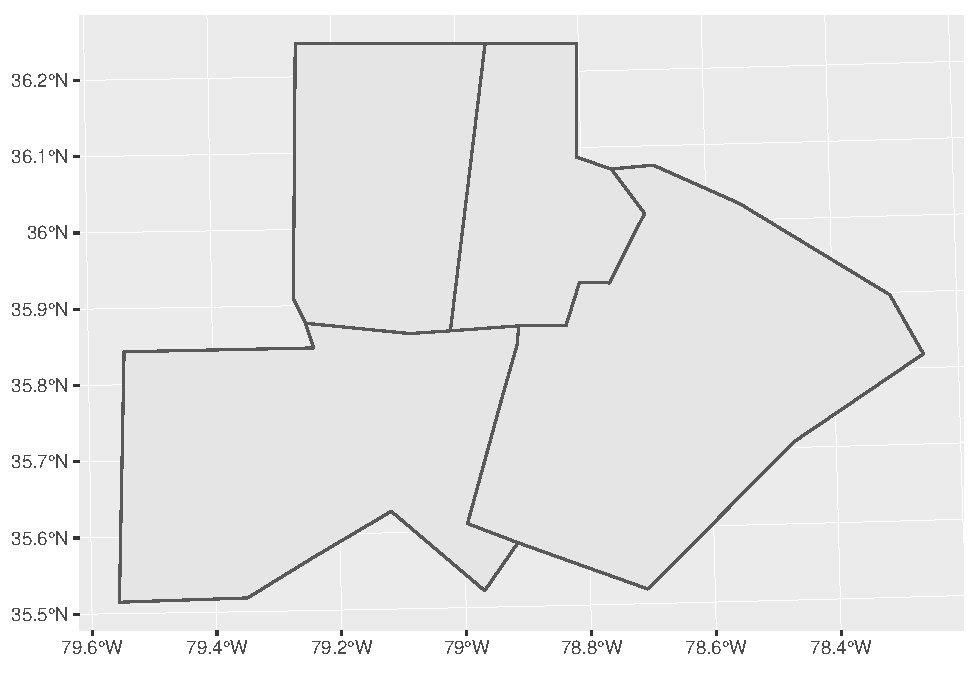
\includegraphics{14_TimeSeries_files/figure-latex/unnamed-chunk-2-1.pdf}

\begin{Shaded}
\begin{Highlighting}[]
\CommentTok{# Split dataset by lake}
\NormalTok{Peter.nutrients.surface <-}\StringTok{ }\KeywordTok{filter}\NormalTok{(PeterPaul.nutrients.surface, lakename }\OperatorTok{==}\StringTok{ "Peter Lake"}\NormalTok{)}
\NormalTok{Paul.nutrients.surface <-}\StringTok{ }\KeywordTok{filter}\NormalTok{(PeterPaul.nutrients.surface, lakename }\OperatorTok{==}\StringTok{ "Paul Lake"}\NormalTok{)}

\CommentTok{# Paul lake is control. We want to see if they have diff trends.}

\CommentTok{# Run a Mann-Kendall test}
\KeywordTok{mk.test}\NormalTok{(Peter.nutrients.surface}\OperatorTok{$}\NormalTok{tp_ug)}
\end{Highlighting}
\end{Shaded}

\begin{verbatim}
## 
##  Mann-Kendall trend test
## 
## data:  Peter.nutrients.surface$tp_ug
## z = 4.3966, n = 132, p-value = 1.099e-05
## alternative hypothesis: true S is not equal to 0
## sample estimates:
##            S         varS          tau 
## 2.236000e+03 2.584133e+05 2.587065e-01
\end{verbatim}

\begin{Shaded}
\begin{Highlighting}[]
\CommentTok{#Mann-Kendall trend test}

\CommentTok{#data:  Peter.nutrients.surface$tp_ug                   }
\CommentTok{#z = 4.3966, n = 132, p-value = 1.099e-05              }
\CommentTok{#     Low pvalue. there is a trend over time. z positive. positive trend over time.}
\CommentTok{#alternative hypothesis: true S is not equal to 0      No trend over time}
\CommentTok{#sample estimates:}
\CommentTok{#           S         varS          tau   }
\CommentTok{#2.236000e+03 2.584133e+05 2.587065e-01 }

\CommentTok{#Is there a change point of the trend?}
\end{Highlighting}
\end{Shaded}

However, it looks like there might be a breakpoint in our dataset.
Further, we know that Peter Lake underwent experimental fertilization
starting in May 1993, a perturbation which we might expect to have
induced a regime shift in the ecosystem. In this case, we might want to
find out whether there is a breakpoint, or changepoint, in our dataset.

\subsubsection{Pettitt's Test}\label{pettitts-test}

Pettitt's test is also included in the \texttt{trend} package. This
nonparametric test will determine whether there is a shift in the
central tendency of the time series and will tell us at what point the
changepoint occurs (if it detects one). Note: Pettitt's Test will only
test for one changepoint, and further tests must be run if multiple
change points are suspected.

\begin{Shaded}
\begin{Highlighting}[]
\CommentTok{# Test for change point}
\KeywordTok{pettitt.test}\NormalTok{(Peter.nutrients.surface}\OperatorTok{$}\NormalTok{tp_ug)}
\end{Highlighting}
\end{Shaded}

\begin{verbatim}
## 
##  Pettitt's test for single change-point detection
## 
## data:  Peter.nutrients.surface$tp_ug
## U* = 2767, p-value = 4.92e-09
## alternative hypothesis: two.sided
## sample estimates:
## probable change point at time K 
##                              35
\end{verbatim}

\begin{Shaded}
\begin{Highlighting}[]
\CommentTok{#   Pettitt's test for single change-point detection}

\CommentTok{#data:  Peter.nutrients.surface$tp_ug }
\CommentTok{#U* = 2767, p-value = 4.92e-09}
\CommentTok{#alternative hypothesis: two.sided}
\CommentTok{#sample estimates:}
\CommentTok{#probable change point at time K        # where is the change located. 1993. when the experimet started.}
\CommentTok{#                             35 }



\CommentTok{# Run separate Mann-Kendall for each change point  # to see if there is another change.}
\KeywordTok{mk.test}\NormalTok{(Peter.nutrients.surface}\OperatorTok{$}\NormalTok{tp_ug[}\DecValTok{1}\OperatorTok{:}\DecValTok{34}\NormalTok{]) }\CommentTok{# no significant trend (becaue the change is balancing it)}
\end{Highlighting}
\end{Shaded}

\begin{verbatim}
## 
##  Mann-Kendall trend test
## 
## data:  Peter.nutrients.surface$tp_ug[1:34]
## z = 0.14834, n = 34, p-value = 0.8821
## alternative hypothesis: true S is not equal to 0
## sample estimates:
##            S         varS          tau 
## 1.100000e+01 4.544333e+03 1.971355e-02
\end{verbatim}

\begin{Shaded}
\begin{Highlighting}[]
\KeywordTok{mk.test}\NormalTok{(Peter.nutrients.surface}\OperatorTok{$}\NormalTok{tp_ug[}\DecValTok{35}\OperatorTok{:}\DecValTok{132}\NormalTok{]) }\CommentTok{# no significant trend }
\end{Highlighting}
\end{Shaded}

\begin{verbatim}
## 
##  Mann-Kendall trend test
## 
## data:  Peter.nutrients.surface$tp_ug[35:132]
## z = -1.6329, n = 98, p-value = 0.1025
## alternative hypothesis: true S is not equal to 0
## sample estimates:
##             S          varS           tau 
## -5.330000e+02  1.061503e+05 -1.121397e-01
\end{verbatim}

\begin{Shaded}
\begin{Highlighting}[]
\CommentTok{# Is there a second change point?}
\KeywordTok{pettitt.test}\NormalTok{(Peter.nutrients.surface}\OperatorTok{$}\NormalTok{tp_ug[}\DecValTok{35}\OperatorTok{:}\DecValTok{132}\NormalTok{]) }\CommentTok{# there is a trend change.}
\end{Highlighting}
\end{Shaded}

\begin{verbatim}
## 
##  Pettitt's test for single change-point detection
## 
## data:  Peter.nutrients.surface$tp_ug[35:132]
## U* = 1201, p-value = 0.0002228
## alternative hypothesis: two.sided
## sample estimates:
## probable change point at time K 
##                              79
\end{verbatim}

\begin{Shaded}
\begin{Highlighting}[]
\CommentTok{# Run another Mann-Kendall for the second change point}
\KeywordTok{mk.test}\NormalTok{(Peter.nutrients.surface}\OperatorTok{$}\NormalTok{tp_ug[}\DecValTok{35}\OperatorTok{:}\DecValTok{113}\NormalTok{]) }\CommentTok{#here we detect the trend}
\end{Highlighting}
\end{Shaded}

\begin{verbatim}
## 
##  Mann-Kendall trend test
## 
## data:  Peter.nutrients.surface$tp_ug[35:113]
## z = 2.7432, n = 79, p-value = 0.006084
## alternative hypothesis: true S is not equal to 0
## sample estimates:
##            S         varS          tau 
## 6.490000e+02 5.580033e+04 2.106459e-01
\end{verbatim}

\begin{Shaded}
\begin{Highlighting}[]
\KeywordTok{mk.test}\NormalTok{(Peter.nutrients.surface}\OperatorTok{$}\NormalTok{tp_ug[}\DecValTok{114}\OperatorTok{:}\DecValTok{132}\NormalTok{]) }\CommentTok{#here no trend.}
\end{Highlighting}
\end{Shaded}

\begin{verbatim}
## 
##  Mann-Kendall trend test
## 
## data:  Peter.nutrients.surface$tp_ug[114:132]
## z = 0.62974, n = 19, p-value = 0.5289
## alternative hypothesis: true S is not equal to 0
## sample estimates:
##           S        varS         tau 
##  19.0000000 817.0000000   0.1111111
\end{verbatim}

\begin{Shaded}
\begin{Highlighting}[]
\CommentTok{# Run the same test for Paul Lake. }
\KeywordTok{mk.test}\NormalTok{(Paul.nutrients.surface}\OperatorTok{$}\NormalTok{tp_ug) }\CommentTok{#non significant}
\end{Highlighting}
\end{Shaded}

\begin{verbatim}
## 
##  Mann-Kendall trend test
## 
## data:  Paul.nutrients.surface$tp_ug
## z = -1.4366, n = 131, p-value = 0.1508
## alternative hypothesis: true S is not equal to 0
## sample estimates:
##             S          varS           tau 
## -7.230000e+02  2.525897e+05 -8.498887e-02
\end{verbatim}

\begin{Shaded}
\begin{Highlighting}[]
\KeywordTok{pettitt.test}\NormalTok{(Paul.nutrients.surface}\OperatorTok{$}\NormalTok{tp_ug) }\CommentTok{#non significant}
\end{Highlighting}
\end{Shaded}

\begin{verbatim}
## 
##  Pettitt's test for single change-point detection
## 
## data:  Paul.nutrients.surface$tp_ug
## U* = 1024, p-value = 0.1244
## alternative hypothesis: two.sided
## sample estimates:
## probable change point at time K 
##                              58
\end{verbatim}

\begin{Shaded}
\begin{Highlighting}[]
\CommentTok{# Add vertical lines to the original graph to represent change points}
\KeywordTok{ggplot}\NormalTok{(PeterPaul.nutrients.surface, }\KeywordTok{aes}\NormalTok{(}\DataTypeTok{x =}\NormalTok{ sampledate, }\DataTypeTok{y =}\NormalTok{ tp_ug, }\DataTypeTok{color =}\NormalTok{ lakename)) }\OperatorTok{+}\StringTok{ }
\StringTok{  }\KeywordTok{geom_point}\NormalTok{() }\OperatorTok{+}
\StringTok{  }\KeywordTok{scale_color_manual}\NormalTok{(}\DataTypeTok{values =} \KeywordTok{c}\NormalTok{(}\StringTok{"#7fcdbb"}\NormalTok{, }\StringTok{"#253494"}\NormalTok{)) }\OperatorTok{+}
\StringTok{  }\KeywordTok{geom_vline}\NormalTok{(}\DataTypeTok{xintercept=}\KeywordTok{as.Date}\NormalTok{(}\StringTok{"1993/05/20"}\NormalTok{), }\DataTypeTok{color=} \StringTok{"#253494"}\NormalTok{, }\DataTypeTok{lty=}\DecValTok{2}\NormalTok{) }\OperatorTok{+}
\StringTok{   }\KeywordTok{geom_vline}\NormalTok{(}\DataTypeTok{xintercept=}\KeywordTok{as.Date}\NormalTok{(}\StringTok{"1998/01/01"}\NormalTok{), }\DataTypeTok{color=} \StringTok{"#253494"}\NormalTok{, }\DataTypeTok{lty=}\DecValTok{2}\NormalTok{)}
\end{Highlighting}
\end{Shaded}

\includegraphics{14_TimeSeries_files/figure-latex/unnamed-chunk-3-1.pdf}

\begin{Shaded}
\begin{Highlighting}[]
  \CommentTok{#+ scale_y_log10() use when you have realy low and high values.}
\CommentTok{#you can do sense slope to quantify the slope}
\end{Highlighting}
\end{Shaded}

\subsubsection{Seasonal Mann-Kendall}\label{seasonal-mann-kendall}

Like a \textbf{Mann-Kendall Test}, the \textbf{Seasonal Mann-Kendall
Test}, or \textbf{Hirsch-Slack Test}, analyzes trends in response
variables over time. It replaces the traditional Mann-Kendall when there
are seasonal trends in a dataset that obscure the overall direction of
the trend. It is important to note that ``seasonal'' does not
necessarily equate to actual seasons but can represent any time period
within which there are oscillating temporal trends. The test needs at
least two seasons to operate.

For instance, we might want to know whether there is a change in
discharge of the Eno River over the last 10 years.

\begin{Shaded}
\begin{Highlighting}[]
\CommentTok{# Wrangle the USGS dataset}
\NormalTok{USGS.flow.data.trimmed <-}\StringTok{ }\NormalTok{USGS.flow.data }\OperatorTok
\StringTok{  }\KeywordTok{select}\NormalTok{(datetime, discharge.mean) }\OperatorTok
\StringTok{  }\KeywordTok{filter}\NormalTok{(datetime }\OperatorTok{>}\StringTok{ }\KeywordTok{as.Date}\NormalTok{(}\StringTok{"2008-12-31"}\NormalTok{) }\OperatorTok{&}\StringTok{ }\NormalTok{datetime }\OperatorTok{<}\StringTok{ }\KeywordTok{as.Date}\NormalTok{(}\StringTok{"2019-01-01"}\NormalTok{))}

\CommentTok{# Visualize the data}
\KeywordTok{ggplot}\NormalTok{(USGS.flow.data.trimmed, }\KeywordTok{aes}\NormalTok{(}\DataTypeTok{x =}\NormalTok{ datetime, }\DataTypeTok{y =}\NormalTok{ discharge.mean)) }\OperatorTok{+}
\StringTok{  }\KeywordTok{geom_point}\NormalTok{(}\DataTypeTok{size =} \FloatTok{0.5}\NormalTok{, }\DataTypeTok{alpha =} \FloatTok{0.5}\NormalTok{)}
\end{Highlighting}
\end{Shaded}

\begin{verbatim}
## Warning: Removed 16 rows containing missing values (geom_point).
\end{verbatim}

\includegraphics{14_TimeSeries_files/figure-latex/unnamed-chunk-4-1.pdf}

\subsubsection{Interpolation}\label{interpolation}

Some situations may require us to predict values for data points that
fall within the time frame of our analyses but were not sampled. For
instance, the \texttt{smk.test} function needs to take a time series
format rather than a data frame, which cannot have any NAs. In this
case, we will want to make an estimate of the missing values based on
what we know about the dataset using a method called
\textbf{interpolation.} There are several options for interpolation:

\begin{itemize}
\item
  \textbf{Means interpolation:} Defines values between sampled values as
  the mean value within a dataset. Uses the R function
  \texttt{aggregate}.
\item
  \textbf{Piecewise constant interpolation:} Defines values between
  sampled values as the value of the nearest sampled value. Uses the R
  function \texttt{approx} with \texttt{method\ =\ "constant"}
\item
  \textbf{Linear interpolation:} Defines values between sampled values
  based on the slope between sampled values. Uses the R function
  \texttt{approx} with \texttt{method\ =\ "linear"}
\item
  \textbf{Spline interpolation:} Defines values between sampled values
  based on polynomial functions between sampled values and chooses the
  polynomials so that they fit smoothly together. Uses the R function
  \texttt{splinefun}.
\end{itemize}

Question: Under what circumstances would you consider each of these
options for interpolation?

\begin{quote}
ANSWER: Linear. because continues data.
\end{quote}

Tip: Check your dataset to see if there is an NA value in the first row.
You may need to add a value for that first row or trim the dataset so
that the new first row corresponds to the first measurement.

\begin{Shaded}
\begin{Highlighting}[]
\CommentTok{# Run a linear interpolation of the dataset to fill in gaps}
\NormalTok{USGS.flow.data.interpolated <-}\StringTok{ }\KeywordTok{approx}\NormalTok{(USGS.flow.data.trimmed}\OperatorTok{$}\NormalTok{datetime,}
\NormalTok{                                      USGS.flow.data.trimmed}\OperatorTok{$}\NormalTok{discharge.mean, }
                                      \DataTypeTok{method =} \StringTok{"linear"}\NormalTok{, }\DataTypeTok{n =} \DecValTok{3630}\NormalTok{) }
\CommentTok{# so you dont generate new points. I think this was to fill rows with NAs. It give us a list.}

\CommentTok{# Turn the interpolated dataset into a proper dataframe}
\NormalTok{USGS.flow.data.interpolated <-}\StringTok{ }\KeywordTok{do.call}\NormalTok{(cbind.data.frame, USGS.flow.data.interpolated)}
\KeywordTok{names}\NormalTok{(USGS.flow.data.interpolated) <-}\StringTok{ }\KeywordTok{c}\NormalTok{(}\StringTok{"Date"}\NormalTok{, }\StringTok{"Discharge"}\NormalTok{)}
\NormalTok{USGS.flow.data.interpolated}\OperatorTok{$}\NormalTok{Date <-}\StringTok{ }\KeywordTok{as.Date}\NormalTok{(USGS.flow.data.interpolated}\OperatorTok{$}\NormalTok{Date, }
                                            \DataTypeTok{origin =} \StringTok{"1970/01/01"}\NormalTok{)}

\CommentTok{# Create a time series object FRA: we need this for the seasonal test.}
\NormalTok{USGS.flow.data.timeseries <-}\StringTok{ }\KeywordTok{ts}\NormalTok{(USGS.flow.data.interpolated}\OperatorTok{$}\NormalTok{Discharge, }
                                \DataTypeTok{start =} \KeywordTok{c}\NormalTok{(}\DecValTok{2009}\NormalTok{, }\DecValTok{1}\NormalTok{) ,}\DataTypeTok{frequency =} \DecValTok{12}\NormalTok{) }
\CommentTok{#12 beacuse is monthly. you can out 365.}

\CommentTok{# Run a Seasonal Mann-Kendall test}
\NormalTok{USGS.smktest <-}\StringTok{ }\KeywordTok{smk.test}\NormalTok{(USGS.flow.data.timeseries)}
\NormalTok{USGS.smktest }\CommentTok{# overall trend. similar to the first test that we did. pvalue low, there is a trend.}
\end{Highlighting}
\end{Shaded}

\begin{verbatim}
## 
##  Seasonal Mann-Kendall trend test (Hirsch-Slack test)
## 
## data:  USGS.flow.data.timeseries
## z = 7.6477, p-value = 2.047e-14
## alternative hypothesis: true S is not equal to 0
## sample estimates:
##        S     varS 
##    46576 37089370
\end{verbatim}

\begin{Shaded}
\begin{Highlighting}[]
\KeywordTok{summary}\NormalTok{(USGS.smktest) }\CommentTok{#gives as each month. the trends each season. Season 11 biggest trend. }
\end{Highlighting}
\end{Shaded}

\begin{verbatim}
## 
##  Seasonal Mann-Kendall trend test (Hirsch-Slack test)
## 
## data: USGS.flow.data.timeseries
## alternative hypothesis: two.sided
## 
## Statistics for individual seasons
## 
## H0
##                       S    varS   tau     z   Pr(>|z|)    
## Season 1:   S = 0  4158 3106080 0.091 2.359 0.01833881   *
## Season 2:   S = 0  3495 3106087 0.076 1.983 0.04742183   *
## Season 3:   S = 0  2907 3106086 0.064 1.649 0.09917234   .
## Season 4:   S = 0  2614 3106083 0.057 1.483 0.13817263    
## Season 5:   S = 0  2762 3106073 0.060 1.567 0.11720613    
## Season 6:   S = 0  3381 3106074 0.074 1.918 0.05513217   .
## Season 7:   S = 0  2982 3075479 0.066 1.700 0.08916281   .
## Season 8:   S = 0  4417 3075480 0.097 2.518 0.01179905   *
## Season 9:   S = 0  3984 3075481 0.088 2.271 0.02313537   *
## Season 10:   S = 0 5431 3075484 0.120 3.096 0.00195952  **
## Season 11:   S = 0 5921 3075481 0.130 3.376 0.00073625 ***
## Season 12:   S = 0 4524 3075485 0.100 2.579 0.00990553  **
## ---
## Signif. codes:  0 '***' 0.001 '**' 0.01 '*' 0.05 '.' 0.1 ' ' 1
\end{verbatim}

\begin{Shaded}
\begin{Highlighting}[]
\CommentTok{# No trend in season 5 for example}
\end{Highlighting}
\end{Shaded}

Interpreting results of the Seasonal Mann-Kendall Test:

\begin{itemize}
\item
  Overall z score and p-value: test the alternative hypothesis that the
  true change in response variable over time is not equal to zero
\item
  Monthly z score and p-value: test the alternative hypothesis that the
  true change in response variable over time for a given month is not
  equal to zero
\item
  S: reports trend. A positive value indicates response variable
  increased over time, and a negative value indicates response variable
  decreased over time
\end{itemize}

Question: How would you interpret the results of the Seasonal
Mann-Kendall test for this example?

\begin{quote}
ANSWER:
\end{quote}


\end{document}
